\FloatBarrier
\section{Causal Training from Saved Quantized Operands}
\label{sec:causal-training}

Training adds three constraints to the forward problem.  Causal attention
masks future tokens, grouped-query attention (GQA) lets several query heads
share key/value heads, and backward must recover gradients without
materializing the full $S\times S$ score or probability matrices.  We first
present the retained method, then measure isolated backward,
projection-inclusive attention, a complete model update, and distributed
training.  Rejected designs remain in
Appendix~\ref{app:causal-design-history}.

\subsection{Pass the forward quantization into backward}

The forward pass saves the NVFP4 query/key payload bytes, their block scales,
the per-head Q--K global factors, and each row's log-sum-exp (LSE)
normalizer.  Backward recomputes $QK^\mathsf{T}$ from those bytes and scales,
then uses LSE to reconstruct the probabilities.  Separately, the projection
epilogue publishes row- or column-oriented FP8 views of Q, K, and V so each
gradient matrix product receives its required physical layout without a
standalone transpose or quantization launch.  Thus ``exact'' below means
exact with respect to the quantized forward payload, not to unquantized BF16
inputs.  Row-oriented and column-oriented describe how the same represented
values and scales are arranged for different matrix instructions; they do not
introduce a second quantization rule.

The implementation dispatches the Llama-style
8-billion-parameter attention shape at local batch sizes
$B\in\{1,2,4\}$, sequence length $S=4096$, 32 query heads, eight key/value
heads, and head dimension $D=128$.
The combined
query/key/value (QKV) projection applies rotary positional embedding (RoPE) and
publishes the layouts needed by forward and backward while its output fragments
are still live.  This avoids launching separate quantization and transpose
kernels around every attention layer.

This is not pure-FP4 end-to-end training.  Learned projections and attention
are separate precision boundaries.  We evaluate E4M3 projections as a
numerical control and NVFP4 projections as the higher-throughput arm.  Inside
attention, the controlled format comparison selects FP8 rather than MXFP4 for
P and V.  The supporting ablations are collected in
Appendix~\ref{app:causal-design-history}.

We prefix a tensor with d to denote its gradient; dO is the gradient arriving
from the output projection.

\begin{table}[htbp]
\centering
\caption{Precision contract for causal training.  Learned projections and
attention operands are separate boundaries.}
\label{tab:causal-precision-contract}
\small
\begin{tabularx}{\textwidth}{p{.25\textwidth}p{.27\textwidth}X}
\toprule
Part of the model & Representation & Reason \\
\midrule
Learned QKV and output projections & E4M3 control or NVFP4 throughput arm;
FP32 accumulation & Separates projection error from the attention-format
comparison. \\
Forward score product & NVFP4 Q and K & Reuses two-dimensional scales over
16-value blocks along the inner dimension (row-by-K16). \\
Forward value product & FP8 P and V & Retained training route; the MXFP4
alternative is faster in isolation but diverges in the observed distributed
experiments. \\
Probability reconstruction in backward & Saved NVFP4 Q/K, block and global
scales, and LSE &
Reconstructs the same represented probability used by forward without storing
an $S\times S$ matrix. \\
Backward gradient products & E4M3 Q/K/V/P/dS; E5M2 dO & E4M3 supplies
precision; E5M2 supplies the range needed for the small output gradient dO. \\
Gradient outputs & FP32 accumulation, BF16 dQ/dK/dV & Keeps accumulation and
optimizer-facing gradients stable. \\
\bottomrule
\end{tabularx}
\end{table}
\FloatBarrier

\subsection{How the backward pass works}

We write dQ, dK, dV, dP, and dS for gradients of the corresponding attention
tensors.  The backward pass executes five tiled matrix products, beginning
with $QK^\mathsf{T}$ reconstructed from the saved quantized operands:
\begin{equation}
  dP=dO\,V^\mathsf{T},\qquad
  dV=P^\mathsf{T}dO,\qquad
  dQ=dS\,K,\qquad
  dK=dS^\mathsf{T}Q.
  \label{eq:causal-bwd-products}
\end{equation}
The softmax gradient is
\begin{equation}
  r_i=\langle O_i,dO_i\rangle,\qquad
  dS=P\odot(dP-r\mathbf 1^\mathsf{T}),
  \label{eq:causal-bwd-ds}
\end{equation}
so probability reconstruction and dP must both complete before dQ and dK can
begin.  Causal masking removes illegal tiles but also makes work ownership
uneven.

\begin{figure}[H]
\centering
\begin{tikzpicture}[
  font=\scriptsize,
  block/.style={draw=inkgray,rounded corners=2pt,align=center,
    minimum width=2.25cm,minimum height=.72cm,inner sep=3pt},
  edge/.style={-{Latex[length=1.8mm]},thick,draw=inkgray}]
  \node[block,fill=scaleyellow!20] (do) at (3.0,3.0) {output gradient\\E5M2 dO};
  \node[block,fill=scoreblue!18] (scorein) at (0,1.8)
    {saved NVFP4 Q/K\\scales and LSE};
  \node[block,fill=probred!18] (prob) at (3.0,1.8)
    {form $QK^\mathsf{T}$\\reconstruct P};
  \node[block,fill=outputgreen!18] (dv) at (6.0,1.8)
    {$dV=P^\mathsf{T}dO$};

  \node[block,fill=scaleyellow!14] (vin) at (0,.6) {saved E4M3 V};
  \node[block,fill=scaleyellow!24] (dp) at (3.0,.6)
    {$dP=dO\,V^\mathsf{T}$};
  \node[block,fill=probred!24] (ds) at (6.0,.6)
    {center and form dS\\publish two layouts};
  \node[block,fill=outputgreen!22] (dq) at (9.0,1.2)
    {$dQ=dS\,K$};
  \node[block,fill=outputgreen!18] (dk) at (9.0,0)
    {$dK=dS^\mathsf{T}Q$};

  \node[block,fill=lightgray] (oin) at (0,-.65) {saved O and dO};
  \node[block,fill=lightgray] (row) at (3.0,-.65)
    {$r_i=\langle O_i,dO_i\rangle$};

  \draw[edge] (scorein) -- (prob);
  \draw[edge] (prob) -- (dv);
  \draw[edge] (do) -- (dv);
  \draw[edge] (do) -- (dp);
  \draw[edge] (vin) -- (dp);
  \draw[edge] (prob) -- (ds);
  \draw[edge] (dp) -- (ds);
  \draw[edge] (oin) -- (row);
  \draw[edge] (row) -- (ds);
  \draw[edge] (ds) -- (dq);
  \draw[edge] (ds) -- (dk);
\end{tikzpicture}
\caption{Causal backward from saved quantized operands.  The serial dependency
runs from probability reconstruction and dP through dS to dQ/dK.  The dV
branch also consumes P and dO, while the saved output and dO provide the
row-centering statistic.  The
equations inside the output boxes name Q/K inputs that are not drawn as extra
crossing arrows.}
\label{fig:causal-backward-dag}
\end{figure}

The implementation accelerates this graph in four ways:
\begin{enumerate}
  \item reconstruct scores from the compact forward payload rather than
  creating a separate BF16 score path;
  \item reuse the rounded P representation for dV and dS instead of decoding
  it twice;
  \item publish both physical dS layouts from the producer fragment and
  release aliased tensor memory as soon as the next consumer owns it; and
  \item publish dO directly as E5M2.  E4M3 rounded roughly 97\% of the observed
  dO values to zero in the failing checkpoint diagnostic, whereas E5M2
  reduced the zero fraction to roughly 14\% with less than 1\% publisher
  overhead.
\end{enumerate}

The D128 backward remains schedule-limited and allows only one CTA per
streaming multiprocessor.  Detailed occupancy and activity counters exist only
for a predecessor schedule, so they are kept with that schedule's timings in
Appendix~\ref{app:causal-design-history} rather than attributed to the retained
binary.

\subsection{Isolated backward}

Does passing the saved quantization into backward make the kernel itself
faster?  We first time only causal attention backward at the production head
dimension,
$D=128$, on one GB200.  Both paths are prepared and bound before timing.  The
BF16 control decodes the same represented E4M3 Q, K, V, and E5M2 dO
operands, whereas the quantized path uses the NVFP4 Q/K payload saved by
forward.  Projection, allocation, loss, and optimizer work
are outside this boundary.

\begin{table}[htbp]
\centering
\caption{Isolated D128 causal backward at B1/S4096.  Latency is the median of
warmed runs; speedup is BF16 latency divided by the latency in each row.}
\label{tab:causal-backward-isolated}
\small
\begin{tabular}{lrr}
\toprule
Route & Latency (ms) & Speedup \\
\midrule
BF16 FA4 backward & 0.501 & 1.000$\times$ \\
Saved-Q/K reconstruction core & 0.356 & 1.405$\times$ \\
Core + E5M2 dO/statistics publisher & 0.508 & 0.986$\times$ \\
\bottomrule
\end{tabular}
\end{table}
\FloatBarrier

The reconstruction core saves 29\% of the BF16 backward time, but the
training-safe E5M2 dO and row-statistic publisher consumes almost exactly that
saving.  This is why a fast backward kernel alone does not predict an
end-to-end gain.  The core passes the exact-zero-dO test, returns finite
nonzero gradients for a nonzero dO, and passes its represented-operand
reference gate.  In the
paired projection-inclusive check, output and input-gradient cosine against
BF16 are 0.998 and 0.956; Q, K, V, and output-projection weight-gradient
cosines range from 0.983 to 0.999.  These are local operator checks, not a
convergence result.

\begin{figure}[H]
\centering
\reportplot[0.20\textheight]{figures/causal_isolated_backward.pdf}
\caption{Isolated D128 causal-backward latency for BF16 and the path that
reconstructs P from saved quantized Q/K at B1/S4096.}
\label{fig:causal-isolated-shape-speedups}
\end{figure}

\Needspace{10\baselineskip}
\subsection{Combined forward and backward}

Does that saving survive its producers and consumers?  The second boundary is
the complete attention sublayer: packed QKV projection,
rotary positional embedding, scale and layout publication, causal attention,
output projection, and their gradients.  It includes the producer and handoff
costs hidden by the isolated kernel test.  It excludes the surrounding root
mean square normalization (RMSNorm), residual connection, language-model
loss, and optimizer.  The BF16 and quantized paths use identical
projection weights and the same B1/S4096/D128 model shape.

\begin{table}[htbp]
\centering
\caption{Projection-inclusive attention on one GB200.  Backward-only runs the
same prepared forward outside the timing interval; the second row times both
forward and backward.  Values are medians of warmed runs.}
\label{tab:causal-combined-forward-backward}
\small
\begin{tabular}{lrrr}
\toprule
Boundary & BF16 (ms) & Quantized route (ms) & Speedup \\
\midrule
Backward only & 1.572 & 1.397 & 1.125$\times$ \\
Forward + backward & 2.656 & 2.133 & 1.245$\times$ \\
\bottomrule
\end{tabular}
\end{table}
\FloatBarrier

\begin{figure}[H]
\centering
\reportplot[0.17\textheight]{figures/causal_combined_forward_backward.pdf}
\caption{Matched projection-inclusive attention forward and backward:
BF16 FA4 versus the saved-quantization path at B1/S4096/D128.}
\label{fig:causal-combined-forward-backward}
\end{figure}

\subsection{Eight-billion-parameter end-to-end result}

Does the attention gain remain visible in a complete model update?  We measure
a full update of a Llama-3.1-style 8.03-billion-parameter
model with 32 layers, 32 query heads, eight key/value heads, and head dimension
128.  We sweep local batch 1, 2, and 4 at sequence length 4096 on one GB200.
Every arm uses the same fused AdamW optimizer and standard dense cross entropy
compiled with \texttt{torch.compile}; cut cross entropy (CCE) is disabled.
Each process is bound to the CPU and memory node local to its GPU.  We report
the median after 10 warmups and 21 measured updates over fixed synthetic
tokens.

The quantized arms use NVFP4 QKV and output projections, row-by-K16 NVFP4
Q/K inside attention, and either FP8 or MXFP4 P/V.  Their backward binary is
identical at a given batch; their forward P/V implementations are
format-specific.  Each quantized measurement is paired with a freshly
measured packed-QKV BF16 FA4 control.

\begin{table}[htbp]
\centering
\caption{Complete 8B updates at S4096 on one GB200.  Each P/V route has its own
adjacent BF16 timing bracket.  Times are medians in milliseconds.}
\label{tab:llama8b-e2e}
\small
\begin{adjustbox}{max width=\textwidth}
\begin{tabular}{rrrrrrr}
\toprule
& \multicolumn{3}{c}{FP8 P/V bracket} & \multicolumn{3}{c}{MXFP4 P/V bracket} \\
\cmidrule(lr){2-4}\cmidrule(lr){5-7}
Local batch & BF16 & Low precision & Speedup & BF16 & Low precision & Speedup \\
\midrule
B1 & 260.313 & 239.985 & 1.085$\times$ & 261.133 & 239.250 & 1.091$\times$ \\
B2 & 464.245 & 415.532 & 1.117$\times$ & 463.814 & 415.408 & 1.117$\times$ \\
B4 & 854.516 & 751.722 & 1.137$\times$ & 857.226 & 751.597 & 1.141$\times$ \\
\bottomrule
\end{tabular}
\end{adjustbox}
\end{table}
\FloatBarrier

The benefit grows as the GPU is better filled: approximately 1.09$\times$ at
B1, 1.12$\times$ at B2, and 1.14$\times$ at B4.  In the FP8 bracket, B4
throughput rises from 19,173 to 21,795 tokens/s per GPU and measured model FLOP
utilization from 41.12\% to 46.74\%.  The MXFP4 arm reaches 21,799 tokens/s and
46.75\% utilization.  FP8 and MXFP4 are therefore tied end to end: their
quantized step times differ by at most 0.31\%, no larger than variation
between their separately measured BF16 anchors.  MXFP4 is modestly faster
in the timed forward portion, but that sub-millisecond difference is not a
material complete-update win.

\begin{figure}[tbp]
\centering
\reportplot[0.19\textheight]{figures/llama8b_e2e_batch_scaling.pdf}
\caption{Complete-update speedup for the two quantized routes as local
batch increases.  These full-route values include NVFP4 QKV/output projections
and therefore are not attention-only or P/V-only speedups.}
\label{fig:llama8b-e2e-breakdown}
\end{figure}

This matrix is deliberately \emph{performance-only}.  Initial-logit cosine
against BF16 is 0.416--0.426 for FP8 P/V and 0.373--0.374 for MXFP4 P/V;
relative-$L_2$ is approximately 1.07 and 1.12.  These short fixed-token updates
do not establish training quality.  The longer FP8 and MXFP4 trajectories in
Appendix~\ref{app:causal-design-history} are separate experiments; a fast
finite timing bracket must not be read as a convergence result.

\subsection{Training stability selects FP8 P/V}

Which probability format remains stable in longer training?  A historical
four-arm diagnostic crossed E4M3 and NVFP4 learned projections with FP8 and
MXFP4 P/V while holding the backward path fixed.  Both FP8-P/V arms remain
non-divergent and descend through their common observed horizon of 55.5
billion tokens.  Both MXFP4-P/V arms separate from their FP8 controls near
0.1 billion tokens and later develop rising loss and very large pre-clipping
gradient norms.  A subsequent matched B4 launch shows the same failure for
NVFP4 projections with MXFP4 P/V: it tracks FP8 through update 300, then its
loss rises from 7.01 at update 325 to 16.25 at update 350.  These experiments
select FP8 P/V for the retained training route.  The complete historical
curves and failure analysis are in
Appendix~\ref{app:causal-design-history}.

\subsection{Matched distributed training}

How do the retained route and BF16 compare at the same training coordinates?
The matched study uses 64 GPUs, local batch four, four gradient
accumulation steps, and effective global batch 1024.  Its BF16 and
NVFP4-projection/FP8-PV arms share the model, optimizer, tokenizer, sample
order, and token schedule.  Both trajectories support exact checkpoint
resume.  We compare them at their latest common coordinate rather than compare
unequal endpoints.  The reporting cutoff for this paper is common update
16,425, corresponding to 68.89 billion tokens in each trajectory.

At that coordinate, BF16 and the FP8 route report losses of 2.3966 and 2.4708
and pre-clipping gradient norms
of 0.0640 and 0.0649, respectively.  At the preceding common held-out
validation, update 16,390, the losses are 2.3507 and 2.4241, a gap of 0.0734.
The FP8 trajectory is therefore stable and descending, but it is not
numerically identical to BF16.  Because the complete route changes both
the learned projections and attention, this comparison does not attribute the
gap to attention alone.  Across all 578 common logged coordinates from the end
of warmup through update 16,425, median throughput is 21,842
tokens/s/GPU for BF16 and 24,287 tokens/s/GPU for the FP8 route; the ratio
of medians is 1.112$\times$.  The paired throughput ratio has a 10th--90th
percentile range of 1.099--1.115$\times$.  This aggregation excludes no
observations, including input stalls and checkpoint windows.  This is one
trajectory per route and therefore does not estimate run-to-run variability.

\begin{figure}[tbp]
\centering
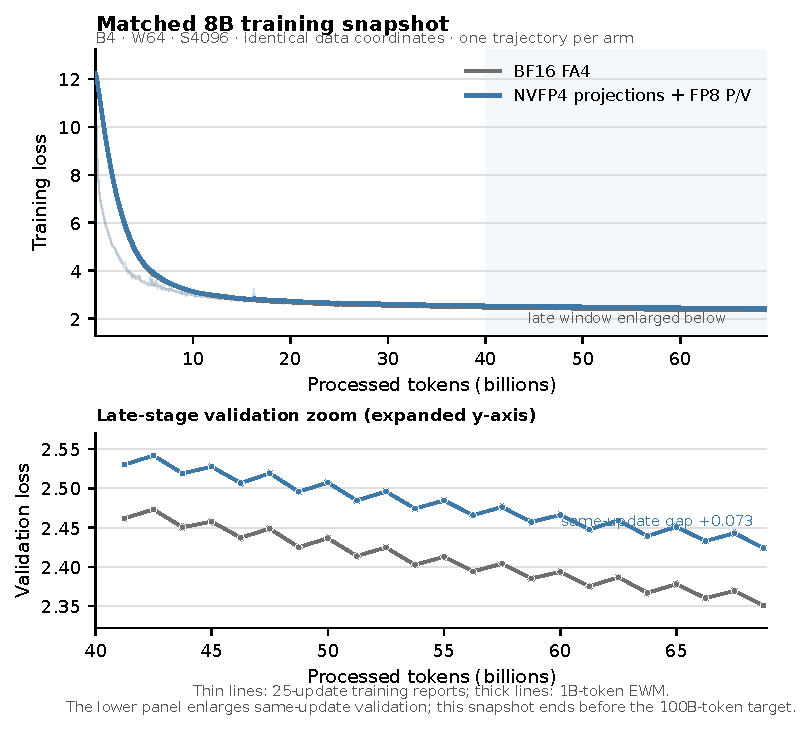
\includegraphics[width=0.82\textwidth]{figures/llama8b_b4_matched_training_curves.pdf}
\caption{Token-aligned training and held-out validation for the matched B4
experiment through the reporting cutoff.  The panel compares the BF16 control
with the retained FP8-P/V route; the lower panel magnifies same-update
validation from 40 billion tokens onward with an expanded vertical axis.
Each curve is one trajectory, so the plot provides no uncertainty estimate.}
\label{fig:llama8b-b4-matched-training}
\end{figure}

\begin{figure}[tbp]
\centering
\reportplot[0.19\textheight]{figures/llama8b_b4_matched_throughput.pdf}
\caption{Distributed throughput for the matched B4 experiment over
all 578 common post-warmup observations.  Input stalls and checkpoint windows
remain in the distribution.}
\label{fig:llama8b-b4-matched-throughput}
\end{figure}
\FloatBarrier

The three local boundaries establish isolated-backward,
projection-inclusive, and full-update speed at D128.  The distributed
evidence establishes the FP8-versus-MXFP4 format choice and includes a
same-recipe BF16 control with same-update validation.  It supports comparisons
through the stated reporting cutoff, but not statistical-equivalence claims
or conclusions about later training coordinates.
